\documentclass[aspectratio=169]{beamer}
%\usetheme{Singapore}
% Load Packages
\usepackage[utf8]{inputenc}
\usepackage{xcolor}
\usepackage{tikz}
\usetikzlibrary{positioning,calc}
\usepackage{graphicx}
\usepackage{hyperref}
\usepackage{amsmath}
\usepackage{listings}
%\usepackage{fontawesome}

\usepackage[sfdefault,light]{FiraSans} %% option 'sfdefault' activates Fira Sans as the default text font
\usepackage[T1]{fontenc}
\renewcommand*\oldstylenums[1]{{\firaoldstyle #1}}

% Define Commands
\newcommand*{\ClipSep}{0.06cm} %To adjust footer logo
\newcommand{\E}{\mathrm{e}\,} %\def\I{e} % used to defined e for exp(x), see later what it should be
\newcommand{\ud}{\mathrm{d}}
\lstset{numbers=left, numberstyle=\tiny, stepnumber=1,firstnumber=1,breaklines=true,
    numbersep=5pt,language=Python,
    stringstyle=\ttfamily,
    basicstyle=\footnotesize, 
    showstringspaces=false
}

\usetheme{oxonian}
\usetheme{Frankfurt}

\title{Dynamic Discrete Choice Models}
\subtitle{An example in Matlab}
\author{
	Shihang Hou
	\and 
	Giulio Schinaia
}
\institute{University of Oxford}
\date{\today}

\setbeamertemplate{navigation symbols}{}

% !TeX spellcheck = en_GB
\usepackage{csquotes}
\usepackage{amsmath}
\usepackage{amsfonts, amssymb}
\usepackage{hyperref}
\usepackage{bm}
\DeclareMathOperator*{\argmax}{arg\,max}
\DeclareMathOperator*{\argmin}{arg\,min}


%%%%%%%%%%%%BLOCK TO UNCOMMENT FOR FINAL VERSION%%%%%%%
% Comment out the next 2 lines for notes version, else uncomment
%\newcommand{\mynoteSH}[1]{}
%\newcommand{\mynoteGS}[1]{}
% Comment following 2 lines for final version, else uncomment
\newcommand{\mynoteSH}[1]{\textcolor{green}{ [SH note: #1]}}
\newcommand{\mynoteGS}[1]{\textcolor{orange}{GS note:[#1]}}

%%Removes navigation symbols
%\setbeamertemplate{navigation symbols}{}

%%Adds page numbers
%\setbeamertemplate{footline}[page number]
\setbeamertemplate{footline}[frame number]{} % sets the frame number instead of the page number (which includes pauses).

\usepackage{csquotes}

\begin{document}
	\begin{frame}
		\titlepage
	\end{frame}
	
	\begin{frame}
		\frametitle{Outline}
		\tableofcontents
	\end{frame}
	
	\section{Overview}
	
	\begin{frame}{Today}
		\begin{itemize}
			\itemsep1em
			%       \item Give an overview of what a dynamic discrete choice model is, and give a sense of what's out there
			%        \item Focus on main elements of single-agent models (the most common)
			%     \pause
			\item Present an example and Matlab code based on \href{https://www.dropbox.com/s/5wn4yj16uhd8s4r/Rust_Optimal\%20Replacement\%20of\%20GMC\%20Bus\%20Engines\%20An\%20Empirical\%20Model\%20of\%20Harold\%20Zurcher_ECMA_1987.pdf?dl=0P}{Rust (1987)}
			\pause
			\item Some concepts are clearly explained on review article by \href{https://www.dropbox.com/s/zvsldc5pmoy1597/Aguirregabiria\%2C\%20Mira_2010_Dynamic\%20discrete\%20choice\%20structural\%20models\%20A\%20survey.pdf?dl=0}{Aguirregabiria and Mira (2010)} (very useful reference!)
		\end{itemize}
	\end{frame}
	
	
	\section{Rust's bus engine replacement model}
	
	\begin{frame}{Overview}
		\begin{itemize}
			\itemsep1em
			\item Based on Rust (1987), Optimal Replacement of GMC Bus Engines: An Empirical Model of Harold Zurcher, Econometrica
			%        \item Harold Zurcher is an employee in a bus company who decides whether to replace a bus engine depending on its current mileage (and other unobserved factors).
			\item One of the first examples of a dynamic discrete choice model (many online code examples R/Julia/Python/Gauss and \textit{now} Matlab for different solution methods available \textemdash 
			check \href{https://sites.google.com/view/victoraguirregabiriaswebsite/computer-code\#h.7dcyjeogndqb}{Aguirregabiria's website} )
			\item     Code is in:\\
			\url{https://github.com/bzdiop/structuralwg/tree/main/presentations/code/SHGS/rust_code}
			There are two sets of scripts:
			\begin{itemize}
				% \itemsep1em
				
				\item finite time horizon (with suffix \texttt{\_finite}) 
				\item infinite time horizon (with suffix \texttt{\_inf}), which we illustrate first, because it is what the paper implements.
				\begin{itemize}
					\item Maybe obvious point: The model assumes the agent makes decisions indefinitely, but the estimation only requires a finite panel.
				\end{itemize}
			\end{itemize}
		\end{itemize}
		
	\end{frame}
	
	\begin{frame}{Harold's problem}
		\begin{itemize}
			\itemsep1em
			\item In each period $t$ and for each bus $b$, Harold has to make a discrete choice $a$:
			\begin{itemize}
				\itemsep1em
				\item to replace the engine of the bus, $a=1$
				\item or not replace the engine, $a=0$.
			\end{itemize}
			\item To make the decision, Harold observes two (types of) state variables:
			\vspace{1em}
			\begin{itemize}
				\itemsep1em
				\item  $x$: Mileage since last replacement (\textbf{Observable} to the researcher)
				\item $\varepsilon$: Reports from the drivers and mechanics, for example. (\textbf{Unobservable} to the researcher)
			\end{itemize}
			
		\end{itemize}
	\end{frame}
	
	
	\begin{frame}{How do we model Harold's behaviour?}\label{utilities}
		
		In each period, we assume the following static utility  \hyperlink{cost.m}{
			\textcolor{gray}{
				\texttt{function}
			}
		}:
		\begin{equation}
			U(x_t,a_t,\theta_1) = \begin{cases}
				- \hspace{1.5cm} c(x_t,\theta_1) + \varepsilon_t(0)  \text{ if } a_t = 0 \\
				-[\overline{P} - \underline{P}+c(0,\theta_1)] + \varepsilon_t(1) \text{ if } a_t = 1
			\end{cases}
		\end{equation}
		
		\begin{itemize}
			\itemsep1em
			\item Standard cost of maintenance depends on mileage: $c(x_t,\theta_1)$, e.g. \hyperlink{c.m}{\textcolor{gray}{\texttt{linear}}}
			\item If replace engine, incur (net) replacement cost (RC) :  $\overline{P}-\underline{P}$ ...
			\item ...but incur lower maintenance costs $c(0,\theta_1)$
			\item Note that we are also making an assumptions about how both the observed and \textit{unobserved} state variables enter the \textbf{additively} in the utility function
		\end{itemize}
		
	\end{frame}
	
	% i as a decision is weird, change in slides
	
	\begin{frame}{(Observable) State variable transition}\label{transprob}
		\begin{itemize}
			\itemsep1em
			\item We also need to make an assumptions about how the state variables evolve over time.
			\item Transition of mileage from period to period is summarised by a stochastic process described by $P(x_{t+1}|x_t,a_t,\theta_2)$
			\item For example, we may \textit{assume} that the gain in mileage is a draw from a \hyperlink{transprob_exponential}{\textcolor{gray}{\texttt{exponential distribution}}}. But this assumption may not fit Harold's data very well (see section III pf the paper).
			\item \textbf{Instead, we assume a more flexible multinomial distribution} to describe how mileage evolves over time (see next slides) given the choice taken in each period.
		\end{itemize}
		
	\end{frame}
	
	\begin{frame}{Create matrix of transition probabilities for all possible states}
		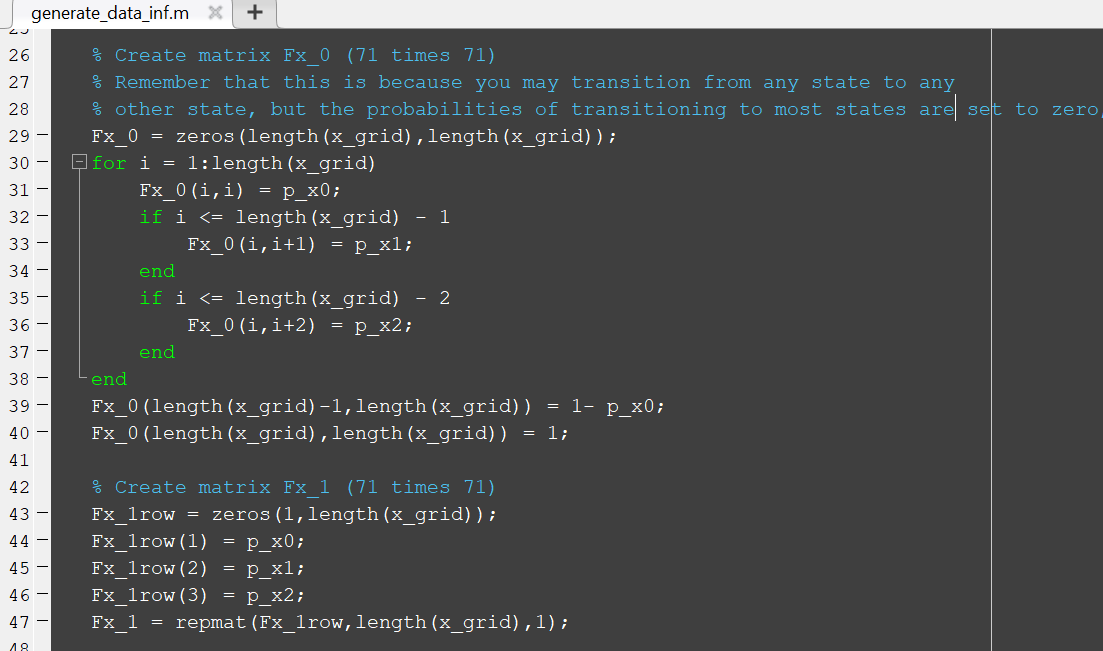
\includegraphics[width=\textwidth]{figs/2_transmat.PNG}
	\end{frame}
	
	\begin{frame}{Matrix of transition probabilities given no replacement}
		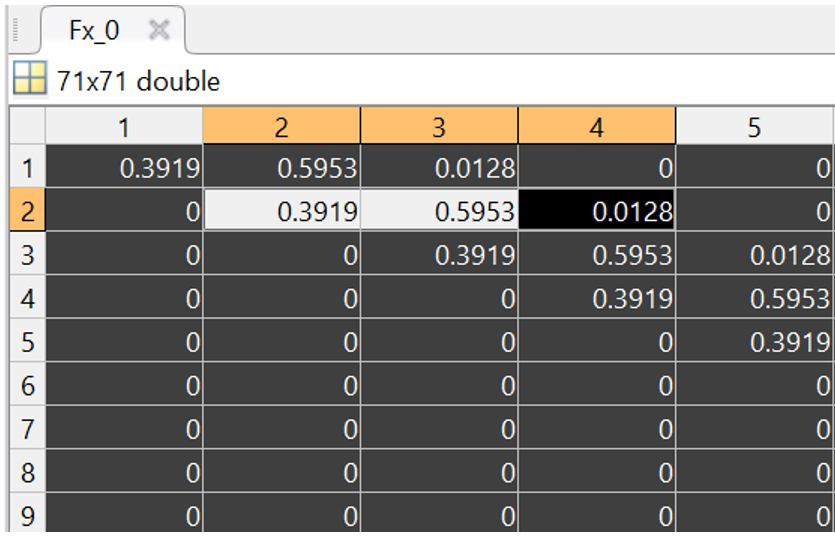
\includegraphics[width=\textwidth]{figs/2_transmat_fx0.PNG}
	\end{frame}
	
	
	\begin{frame}{Matrix of transition probabilities given no replacement}
		
		\begin{itemize}
			\itemsep1em
			\item At zero miles (row 1), there is a 0.3919 probability of only doing 0-5000 miles (cell 1,1), a 0.5953 probability of doing 5001-10000 miles, or a 0.0128 probability of doing 10000-$\infty$ miles.
			\item \textbf{By assumption}, we are bounding the steps to be up to 15000 miles.
			\item This means that there is zero probability of going from zero to beyond 15000 miles.	
			\item There is a zero probability of going back from 5000-10000 to 5000-10000 (cell 2,1).
		\end{itemize}
	\end{frame}
	
	\begin{frame}{What is the goal of the econometrician?}
		%\vspace{1cm}
		\textbf{Goal:} Estimate the paramaters $\theta$ of the model :
		\begin{itemize}
			\itemsep1em
			\item replacement cost
			\item maintenance costs parameters
			\item the transition probabilities for the (observable) state variable
		\end{itemize}
		based on the behavioural model and the econometric assumptions needed to solve it.
	\end{frame}
	
	\begin{frame}{\texttt{generate\_inf.m}: Initialise the parameters to estimate}
		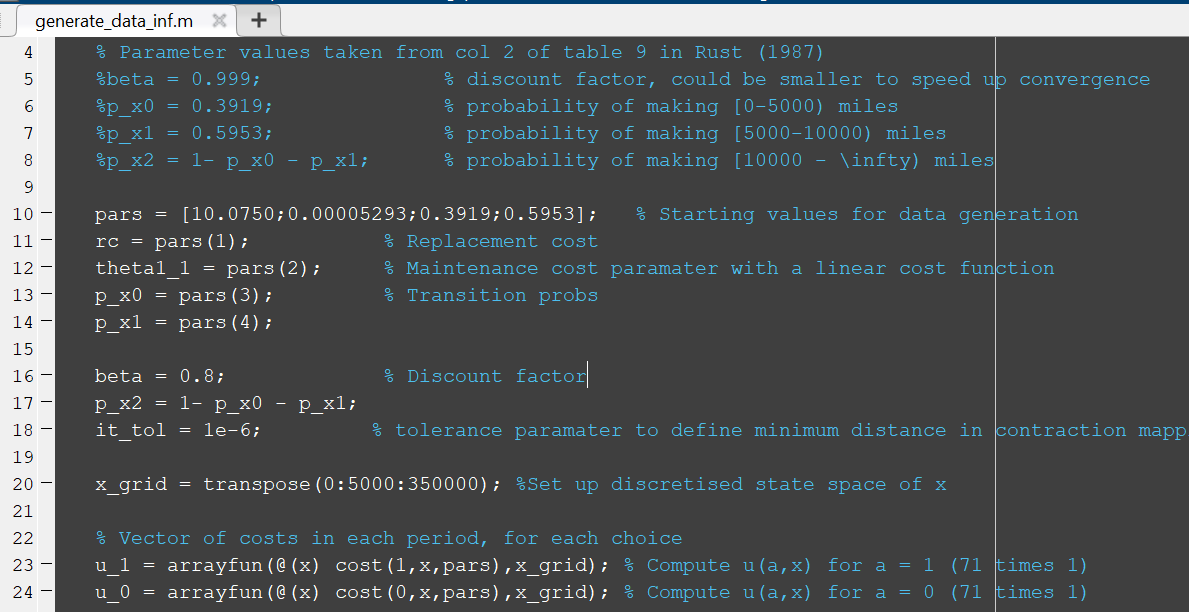
\includegraphics[width=0.9\textwidth]{figs/1_setup.PNG}
	\end{frame}
	
	% give explicit forms we use for the implementation
	
	\begin{frame}{Harold's problem over time}\label{vf}
		\begin{itemize}
			\itemsep1em
			\item Optimal value function (by Bellman's principle): 
			\begin{equation}
				V_\theta(x_t,\varepsilon_t) = \max_{a \in \mathcal{C}(x_t)} [u(x_{t},a,\theta_1) + \varepsilon_t(a) + \beta EV_\theta(x_t,a)]
			\end{equation}
			\item Where the "last term" above is denoted as the Emax function:
			\begin{align}
				EV_\theta(x_t,a) &= \int_{-\infty}^\infty \int_0^\infty V_\theta(y,\varepsilon) p(y|x_t,a,\theta_2) dy dG(\varepsilon) \label{eq:emax_general}
			\end{align}
		\end{itemize}
	\end{frame}
	
	
	
	\begin{frame}{ Rust's \hyperlink{subsec:rust_assumptions}{\textcolor{gray}{assumptions}} (1)}
		\begin{itemize}[<+->]
			\itemsep1em
			\item Thanks to Rust's \hyperlink{subsec:rust_assumptions}{\textcolor{gray}{assumptions}} (IID), (CIX) , we can rewrite \ref{eq:emax_general} as:
			\begin{align}
				EV_\theta(x_t) &= \int \max_{a_t \in \mathcal{C}(x_t)} \left\{ u(a,x_{t}) + \varepsilon_t + \beta \int EV_\theta(x_{t+1})P(x_{t+1}|x_t,a) dx_{t+1} \right\} dG_\varepsilon(\varepsilon_t) \label{eq:emax_rust}
			\end{align}
			\item Usually, would need to compute the double integrals in eq \ref{eq:emax_general}, which would be computationally intensive.
			\item Thanks to Rust's \hyperlink{subsec:rust_assumptions}{\textcolor{gray}{assumption}} (LOGIT), if $\varepsilon$ is distributed according to a type I extreme value distribution, we get:
			\begin{equation}
				EV_\theta(x_t) = \log \left( \sum_{a \in \mathcal{C}(x_t)} \exp \left( u(a,x_t) + \beta  \int EV_\theta(x_{t+1})P(x_{t+1}|x_t,a) dx_{t+1}  \right) \right)
			\end{equation}
		\end{itemize}
	\end{frame}
	
	\begin{frame}{ Rust's \hyperlink{subsec:rust_assumptions}{\textcolor{gray}{assumptions}} (2)}
		\begin{itemize}
			\itemsep1em
			\item For tractability, Rust divides the continuous state space into a discrete set of points.
			\begin{equation} \label{eq:emaxfunc_logit}
				EV_\theta(x_t) = \log \left( \sum_{a \in \mathcal{C}(x_t)} \exp \left( u(a,x_t) + \beta  \sum_{x_{t+1}} EV_\theta(x_{t+1})P(x_{t+1}|x_t,a) \right) \right)
			\end{equation}
			\item For a problem with an infinite time horizon and a finite state space, we can solve for the emax functions as the unique solution to a finite system of equations
			\begin{equation} \label{eq:valuefunciteration}
				\bm{\Bar{V}} = \log \left(\sum_{a=0}^J \exp \left\{ \bm{u}(a,\theta) + \beta \bm{F}_x(a) \bm{\Bar{V}} \right\} \right)
			\end{equation}
		\end{itemize}
	\end{frame}
	
	\begin{frame}{Deriving the Emax values by contraction mapping}
		\begin{itemize}
			\itemsep1em
			\item Rust (1987) shows that equation \ref{eq:emaxfunc_logit} is a contraction mapping from $\bm{\Bar{V}} \rightarrow \bm{\Bar{V}}$.
			\item A straightforward, though computationally complicated approach is to iterate values of the policy functions until the difference between iterations is sufficiently small.
			\begin{equation}\label{eq:emax_iter}
				\bm{\Bar{V}}_{h+1} = \log \left(\sum_{a=0}^J \exp \left\{ \bm{u}(a,\theta) + \beta \bm{F}_x(a) \bm{\Bar{V}}_h \right\} \right)
			\end{equation}
			\item Note: For finite horizon applications, backward induction is most common solution method (see example later).
		\end{itemize}
	\end{frame}
	
	
	\begin{frame}{Iterating the value function}
		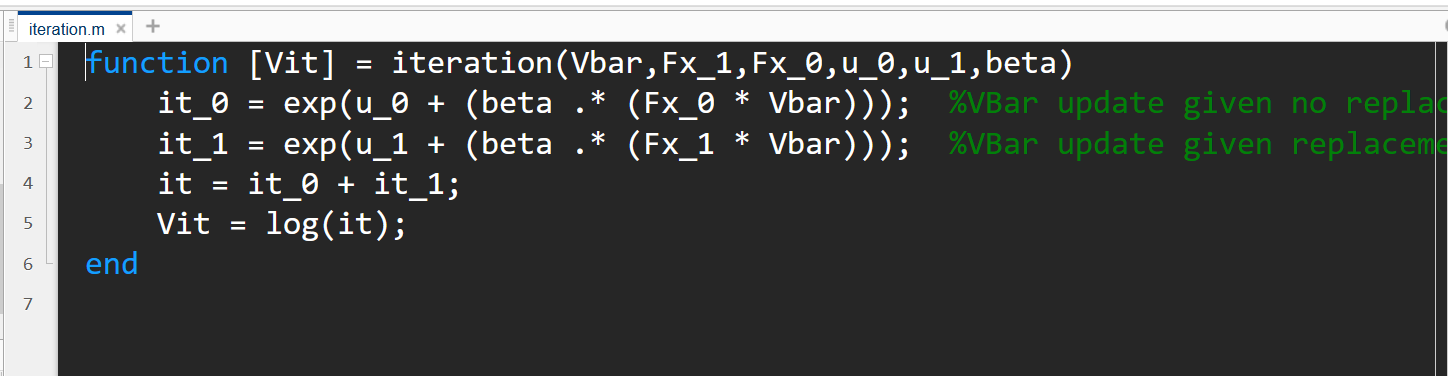
\includegraphics[width=\textwidth]{figs/3_iteration.PNG}
	\end{frame}
	
	%\section{Code Demo 1: Infinite Time Horizon}
	
	
	\begin{frame}{Contraction mapping algorithm to evaluate following \ref{eq:emax_iter}}
		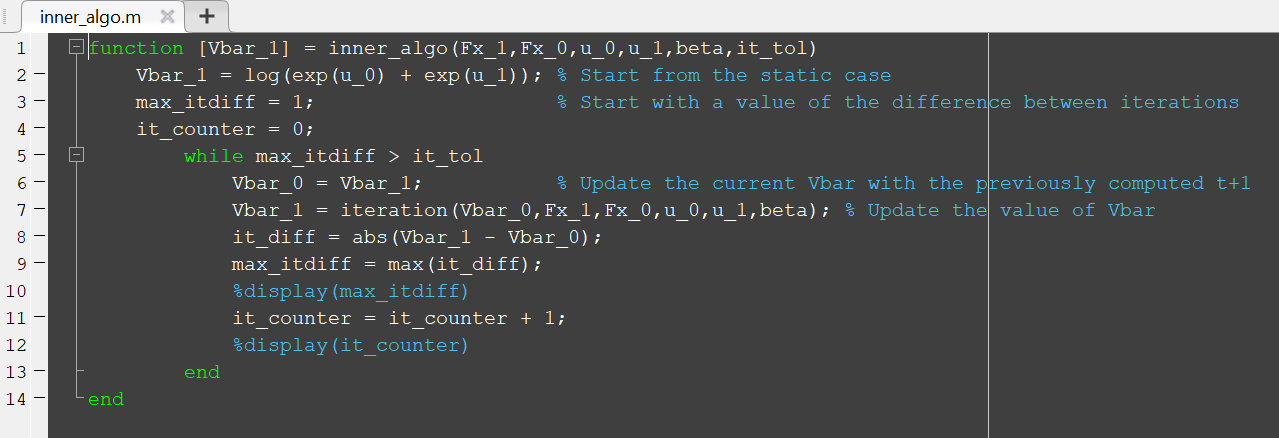
\includegraphics[width=\textwidth]{figs/3_inneralgo.PNG}
	\end{frame}
	
	
	\begin{frame}{Estimation steps of the outer algorithm}
		\begin{enumerate}
			\itemsep1em
			\item Start with guess $\hat{\theta}_0$.
			\item Evaluate $\bm{\Bar{V}}(\hat{\theta}_0)$, either by iteration until convergence using the contraction mapping (see equation \ref{eq:valuefunciteration} or backwards induction for the finite case).
			\item Use $\bm{\Bar{V}}(\hat{\theta}_0)$ and parameter guesses $\hat{\theta}_0$ to compute the choice probability, $P(a|x,\theta)$.
			% \item Use equation \ref{eq:bhhh_iteration} to update the guesses.
			\item Evaluate the log-likelihood and repeat until a local optimum has been reached.
		\end{enumerate}
		
	\end{frame}
	
	\begin{frame}{From the inner to the outer algorithm}
		\texttt{estimate\_inf.m} : Uses the dataset to optimise the log-likelihood function in order to estimate the structural parameters, their standard errors, and confidence intervals.
		
		\begin{itemize}
			\item 	\texttt{rust\_loglik\_inf.m} 
			\begin{enumerate}
				\itemsep1em
				\item performs similar steps as \texttt{generate\_data\_inf.m} to generate the choice probabilities using the inner algorithm, but using different parameters for each iteration of the optimising algorithm.
				\begin{itemize}
					\itemsep1em
					
					\item Uses the same functions to get to the choice probabilities: \texttt{cost.m} , \texttt{c.m} , \texttt{inner\_algo.m}, \texttt{iteration.m} 
				\end{itemize}
				\item Computes the likelihood for the choice probabilities and the transition probability components. 
			\end{enumerate}
			
		\end{itemize}
	\end{frame}
	
	
	
	\begin{frame}{What Rust's assumptions buys us (1) - factorising the log-likelihood}
		\begin{itemize}
			\itemsep1em 
			\item Under CIX and IID, the observable state vector $x_{it}$ is sufficient to determine the current choice, and allows the factorisation of the various terms that enter the log-likelihood contribution. 
			\begin{align} 
				\begin{split} \label{eq:loglik}
					l_i(\theta) = \sum_{t=1}^{T_i} \log(Pr(a_{it}|x_{it},\theta))+  \\
					+ \sum_{t=1}^{T_i - 1}\log(f_X(x_{i,t+1}|a_{it},x_{it},\theta_f))       
				\end{split}
			\end{align}
			
			%  l_i(\theta) = \sum_{t=1}^{T_i} \log(Pr(a_{it}|x_{it},\theta))+ \sum_{t=1}^{T_i} \log(f_Y(y_{it}|a_{it},x_{it},\theta_Y)) \\
			%  + \sum_{t=1}^{T_i - 1}\log(f_X(x_{i,t+1}|a_{it},x_{it},\theta_f)) + \log(Pr(x_{i1}|\theta)) 
			
		\end{itemize}
	\end{frame}
	
	\begin{frame}{Rust's log-likelihood}
		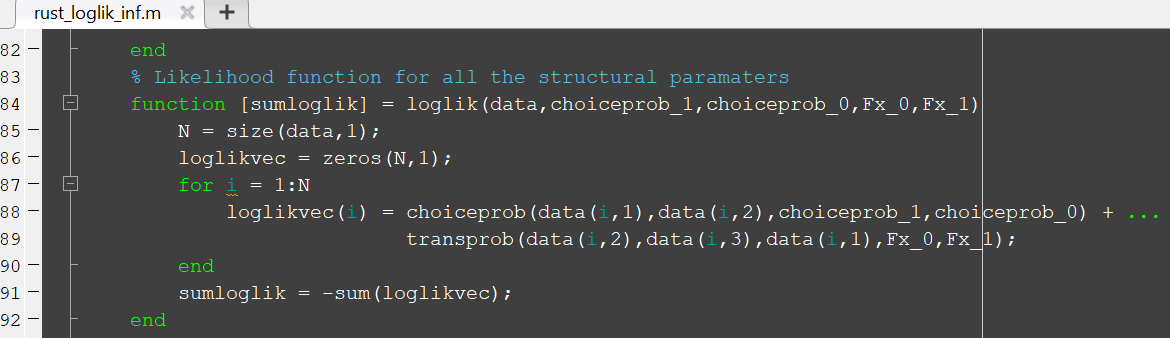
\includegraphics[width=\textwidth]{figs/4_loglik.PNG}\\
		
		\vspace{0.5cm}
		Data contains binary choice to replace in column 1, current mileage in column 2, and next period's mileage in column 3.
	\end{frame}
	
	\begin{frame}{Components of the log-likelihood}
		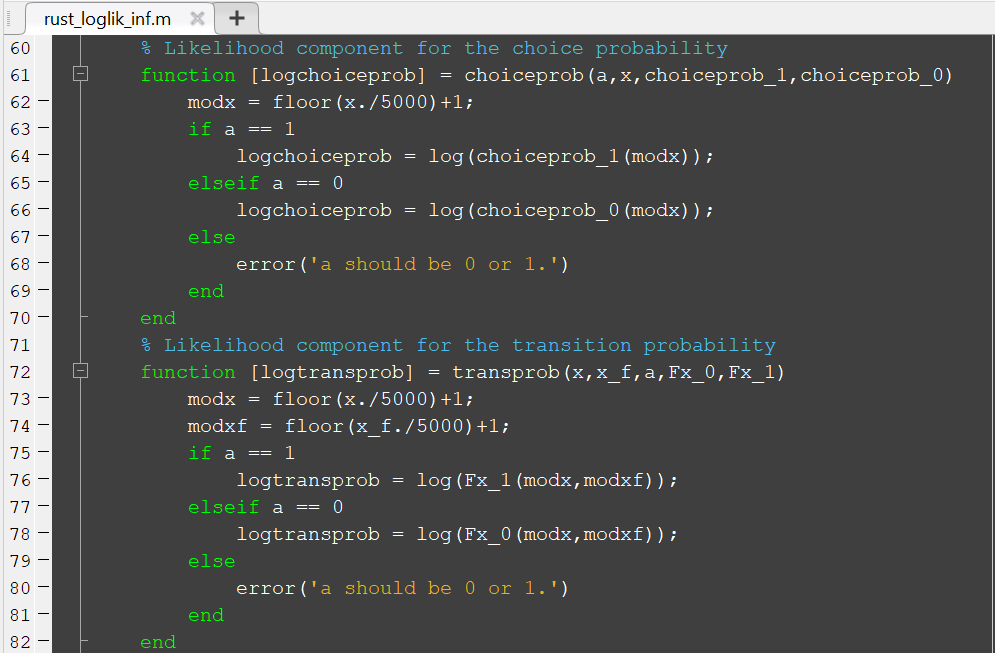
\includegraphics[width=\textwidth]{figs/5_loglik_components.PNG}
	\end{frame}
	
	
	\begin{frame}{What Rust's assumptions buys us (2) - functional form for choice probability}
		\begin{itemize}
			\itemsep1em
			\item Recall the optimal decision rule is $\alpha(x_{it},\varepsilon_{it}) = \argmax_{a \in A} \{v(a,x_{it}) + \varepsilon_{it}(a)\}$, so...
			\begin{align}
				\begin{split}
					Pr(a|x,\theta) &\equiv \int I\{\alpha(x,\varepsilon;\theta) = a\} dG_\varepsilon(\varepsilon) \\
					&= \int I\{v(a,x_{it}) + \varepsilon_{it}(a) > v(a^\prime, x_{it}) + \varepsilon_{it}(a^\prime), \forall a^\prime \neq a\} dG_\varepsilon(\varepsilon_{it}) \\
					&= \frac{\exp(v(a,x))}{\sum_{j=0}^J\exp(v(j,x))}
				\end{split}
			\end{align}
			\item Note slight abuse of notation
			\begin{equation*}
				v(a,x_t) = u(a,x_t) + \beta \sum_{x_{t+1}q \in X} \Bar{V}(x_{t+1}) f_x(x_{t+1}|a,x_t) 
			\end{equation*}
		\end{itemize}
	\end{frame}
	
	
	\begin{frame}{Choice probabilities}
		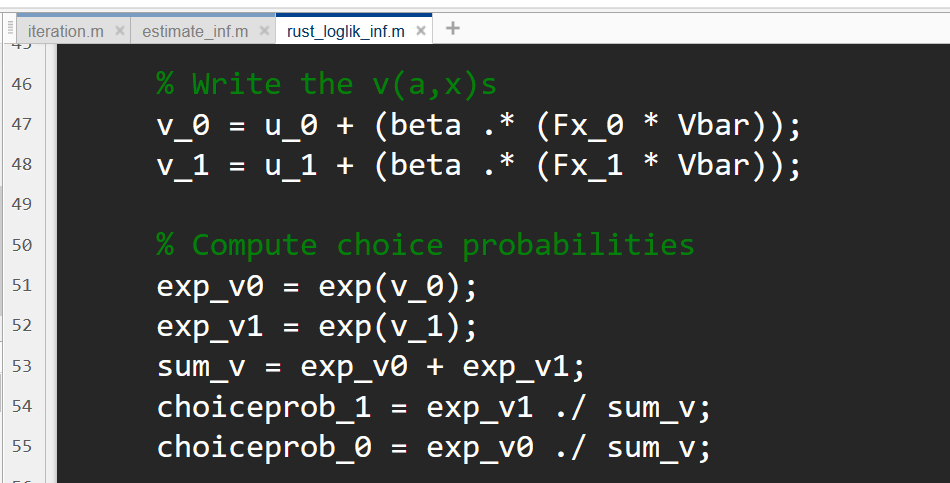
\includegraphics[width=\textwidth]{figs/4_choiceprob.PNG}
	\end{frame}
	
	
	\begin{frame}{Let's run the code}
		...
	\end{frame}
	
	
	\section{Code Demo 2: Finite Time Horizon}
	\begin{frame}{Finite horizon introduction}
		\begin{itemize}
			\itemsep1em
			\item Suppose that a planner runs a bus service, knowing at the start that his franchise ends in 12 periods.
			\item This then becomes a finite time horizon problem, which is typically solved by \textbf{backwards induction}.
		\end{itemize}
	\end{frame}
	\begin{frame}{The final period}
		\begin{itemize}
			\item First, consider the last period $T$. The value of each choice j in T is simply $U_j$, given the value of the state at that time $x_T$. 
			\item The expected value at time T given state value $x_T$ is thus the E-max function:
			\begin{align}
				EV_T(x_T) &= \int \max_{a_T \in \{0,1\}} \left\{ u(x_T,a_T) + \varepsilon_T(a_T) \right\} dG_\varepsilon(\varepsilon_T) \\
				&= \log \left(\sum_{a=0}^J \exp(u_T(a,x_T))\right)
			\end{align}
			\item In matrix form:
			\begin{equation}
				\bar{\bm{V}}_T(\hat{\theta}) = \log \left( \sum_{a=0}^J \exp(\bm{u}_T(a,\hat{\theta}) \right)
			\end{equation}
		\end{itemize}
	\end{frame}
	
	\begin{frame}{The penultimate period ($T-1$)}
		\begin{itemize}
			\itemsep1em
			\item The value of choosing any option $j$ is now $U_j(a_{T-1},x_{T-1}) + \beta \bm{F}_{x,t}(a,x_{T-1}) \bar{\bm{V}}_{T}(\hat{\theta})$.
			\item The expected value at T-1 given state value $x_{T-1}$ is again the E-max function, this time with the implications for the future period included
			\begin{align}
				EV_{T-1}(x_{T-1}) &= \int \max_{a_{T-1} \in \{0,1\}} \left\{ U(x_{T-1},a_{T-1}) + \beta \bm{F}_{x,t}(a,x_{T-1}) \bar{\bm{V}}_{T}(\hat{\theta}) \right\} dG_\varepsilon(\varepsilon_{T-1}) \\
				&= \log \left(\sum_{a=0}^J \exp(u_{T-1}(a,x_{T-1}) + \beta \bm{F}_{x,t}(a,x_{T-1}) \bar{\bm{V}}_{T}(\hat{\theta}))\right)
			\end{align}
		\end{itemize}
	\end{frame}
	
	\begin{frame}{Backwards induction}
		\begin{itemize}
			\itemsep1em
			\item In general, for the Rust assumptions, in matrix form, the values can be solved for recursively using the following expression.
			\begin{equation}
				\Bar{\bm{V}}_t(\hat{\theta}) = \log \left( \sum_{a=0}^J \exp \left\{ \bm{u}_t(a,\hat{\theta}) + \beta \bm{F}_{x,t}(a) \bar{\bm{V}}_{t+1}(\hat{\theta}) \right\} \right)
			\end{equation}
			\item These solved values can then be used to evaluate the probability of observing the given choices:
			\begin{equation}
				Pr_t(a | \hat{\theta}) = \frac{\exp(u_t(a,\hat{\theta}) + \beta \bm{F}_{x,t}(a) \bar{\bm{V}}(\hat{\theta}))}{\sum_{j =0}^J \exp(u_t(j,\hat{\theta}) + \beta \bm{F}_{x,t}(j) \bar{\bm{V}}(\hat{\theta}))}
			\end{equation}
		\end{itemize}
	\end{frame}
	
	\appendix
	\section{Appendix}
	\subsection{Rust models}\label{subsec:rust_assumptions}
	
	\begin{frame}{\hyperlink{vf}{Rust's assumptions (1)}}
		\begin{itemize}
			\itemsep1em
			\item (AS) Additive separability
			\begin{equation*}
				U(a,x_{it},\varepsilon_{it}) = u(a,x_{it}) + \varepsilon_{it}(a)
			\end{equation*}
			\item (CLOGIT) The unobserved state variables $\{\varepsilon_{it}(a): a = 0,1,\cdots,J\}$ are independent across alternatives and have an extreme value type I distribution.
			\item (Discrete support of x) The support of $x_{it}$ is discrete and finite: $x_{it} \in X = \{x^{(1)},x^{(2)},\cdots,x^{(|X|)}\}$ with $|X| < \infty$.
		\end{itemize}
	\end{frame}
	
	\begin{frame}{\hyperlink{vf}{Rust's assumptions (1)}}
		\begin{itemize}
			\itemsep1em
			\item (IID) Unobserved state variables are i.i.d across agents and time, with common cdf $G_\varepsilon(\varepsilon_{it})$
			\item (CIX) Next period observable state variables do not depend on unobserved state variables ($\varepsilon_{it}$)
			$$CDF(x_{it}|x_{it},a_{it},\varepsilon_{it}) = F_x(x_{i,t+1}|a_{it},x_{it})$$
			Denote parameters of $F_x$ by $\theta_f$
			\item CIX + IID $\rightarrow$ $F(x_{i,t+1},\varepsilon_{i,t+1}|a_{it},x_{it},\varepsilon_{it}) = G_\varepsilon(\varepsilon_{i,t+1}) F_x(x_{i,t+1}|a_{it},x_{it})$
		\end{itemize}
	\end{frame}
	
	\begin{frame}{\hyperlink{vf}{Rust's assumptions (3)}}
		\begin{itemize}
			\itemsep1em
			\item (CIY) Conditional on current values of the decision and observable state variables, the value of the payoff variable, $Y$, is independent of $\varepsilon_{it}$
			$$Y(a_{it},x_{it},\varepsilon_{it}) = Y(a_{it},x_{it})$$
			\begin{itemize}
				\item This assumption is not needed in the Rust (1987) example, because we do not have a payoff variable.
			\end{itemize}
		\end{itemize}
	\end{frame}
	
	
	
	\begin{frame}{Some examples of the restrictiveness of Rust's assumptions}
		\begin{itemize}
			\itemsep1em
			\item \textbf{CIX}: Consider an example an observed state variable $x_t$ is human capital and an unobserved state variable is the worker's health $\varepsilon_t$. CIX implies then that health does not affect the rate of accumulation of human capital.
			\item \textbf{CLOGIT and iid}: Choice probabilities exhibit IIA and does not allow for covariance of unobservable state variables - e.g. in occupation choice, unobserved utility are independent between occupations
			\item \textbf{AS}: Implies that marginal utility with respect to observable state variables does not depend on unobservables. e.g. the marginal effect on wage of human capital does not depend on health shocks
		\end{itemize}
	\end{frame}
	
	\begin{frame}{Alternative assumptions (e.g. in Eckstein-Keane-Wolpin models)}
		\begin{itemize}
			\itemsep1em
			\item Relaxing AS by using non-linear functional forms
			\item Observable $Y$ variables that are choice-censored and do not satisfy CIY
			\item Permanent unobserved heterogeneity using mixture models
			\item Unobservables that are correlated across choice options (departing from CLOGIT)
		\end{itemize}
	\end{frame}
	
	
	\begin{frame}{What Rust's assumptions buys us (1) - evaluating the Emax function}
		\begin{itemize}
			\itemsep1em
			\item Fully flexible model
			$$ V(x_{it},\varepsilon_{it}) = \max_{a \in A} \left\{ U(a,x_{it},\varepsilon_{it}) + \beta V(x_{i,t+1},\varepsilon_{i,t+1}) dF(x_{i,t+1},\varepsilon_{i,t+1}|a,x_{it},\varepsilon_{it}) \right\}$$
			\item Rust's model (by AS, CIX, IID, CLOGIT, discrete support)
			\begin{align}
				\Bar{V}(x_{it}) &= \int \max_{a \in A} \left\{ u(a,x_{it}) + \varepsilon_{it}(a) + \beta \sum_{x_{i,t+1} \in X} \Bar{V}(x_{i,t+1})f_x(x_{i,t+1}|a,x_{it}) \right\} dG_\varepsilon(\varepsilon_{it})       \label{eq:Rust_emax_function} \\    
				&= \log \left( \sum_{a=0}^J \exp \left(u(a,x_{it}) + \beta \sum_{x_{i,t+1} \in X} \Bar{V}(x_{i,t+1})f_x(x_{i,t+1}|a,x_{it}) \right)\right)
			\end{align}
			Equation \ref{eq:Rust_emax_function} is known as the Emax function, with a known form for logit errors.
		\end{itemize}
	\end{frame}
	
	\begin{frame}{What Rust's assumptions buys us (2) - factorising the log-likelihood}
		\begin{itemize}
			\itemsep1em 
			\item Under CIX and IID, the observable state vector $x_{it}$ is sufficient to determine the current choice, and allows the factorisation of the various terms that enter the log-likelihood contribution. 
			\begin{align} 
				\begin{split} \label{eq:loglik}
					l_i(\theta) = \sum_{t=1}^{T_i} \log(Pr(a_{it}|x_{it},\theta))+ \sum_{t=1}^{T_i} \log(f_Y(y_{it}|a_{it},x_{it},\theta_Y)) \\
					+ \sum_{t=1}^{T_i - 1}\log(f_X(x_{i,t+1}|a_{it},x_{it},\theta_f)) + \log(Pr(x_{i1}|\theta))           
				\end{split}
			\end{align}
			
		\end{itemize}
	\end{frame}
	
	\begin{frame}{What Rust's assumptions buys us (3) - functional form for choice probability}
		\begin{itemize}
			\itemsep1em
			\item Recall the optimal decision rule is $\alpha(x_{it},\varepsilon_{it}) = \argmax_{a \in A} \{v(a,x_{it}) + \varepsilon_{it}(a)\}$, so...
			\begin{align}
				\begin{split}
					Pr(a|x,\theta) &\equiv \int I\{\alpha(x,\varepsilon;\theta) = a\} dG_\varepsilon(\varepsilon) \\
					&= \int I\{v(a,x_{it}) + \varepsilon_{it}(a) > v(a^\prime, x_{it}) + \varepsilon_{it}(a^\prime), \forall a^\prime \neq a\} dG_\varepsilon(\varepsilon_{it}) \\
					&= \frac{\exp(v(a,x))}{\sum_{j=0}^J\exp(v(j,x))}
				\end{split}
			\end{align}
			\item Note slight abuse of notation
			\begin{equation*}
				v(a,x_t) = u(a,x_t) + \beta \sum_{x_{t+1}q \in X} \Bar{V}(x_{t+1}) f_x(x_{t+1}|a,x_t) 
			\end{equation*}
		\end{itemize}
	\end{frame}
	
	\begin{frame}{\hyperlink{utilities}{Linear costs}}\label{c.m}
		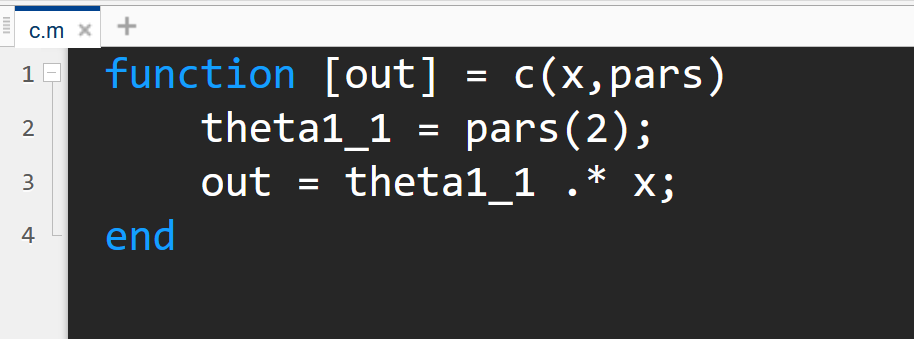
\includegraphics[width=\textwidth]{figs/0_linear_cost.png}\end{frame}
	
	\begin{frame}{\hyperlink{utilities}{Static utilities}}\label{cost.m}
		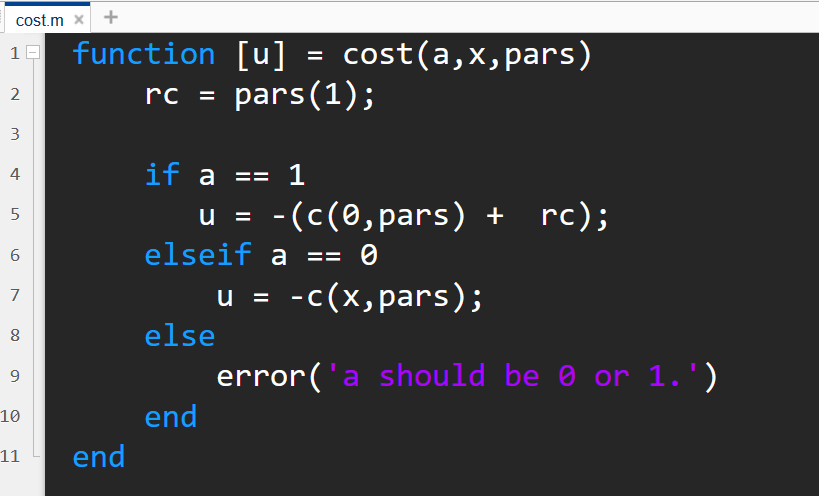
\includegraphics[width=0.8\textwidth]{figs/0_static_utilities.PNG}\end{frame}
	
	\begin{frame}{\hyperlink{state}{State transition probabilities assuming exponential distribution}}\label{transprob_exponential}
		\begin{equation}
			P(x_{t+1}|x_t,a_t,\theta_2) = \begin{cases}
				\theta_2 \exp \{\theta_2 (x_{t+1}-x_t)\} \text{ if } a_t = 0 \text{ and } x_{t+1} \geq x_t \\
				\theta_2 \exp \{\theta_2(x_{t+1})\} \text{ if } a_t = 1 \text{ and } x_{t+1} \geq 0 \\
				0 \text{ otherwise}
			\end{cases}  
		\end{equation}
		\begin{itemize}
			\item Exponential distribution would buy us a closed form solution to the optimal control decision rule, but it is not supported by the data (see Section III of the paper). 
		\end{itemize}
		
	\end{frame}
	
\end{document}


\begin{frame}{Standard choice models}
	\begin{itemize}
		\itemsep1em
		\item For the standard textbook reference, see Train (2009) (recommended by Abi)
		\item Basic idea is to specify a utility for each choice $j \in \{1,\cdots,J\}$ (in the choice set) based on some regular, observable elements of the choice ($u_j$)
		\pause
		\item Total utility for the choice j ($U_j$) is sum of observable component ($u_j$) and a component observed by agent but not the econometrician ($\varepsilon_j$)
		\pause
		\item Choice prob given by:
		\begin{align*}
			Pr(C = j) &= Pr(U_j > U_k , \forall k \neq j) \\
			&= Pr(\varepsilon_j - \varepsilon_k > - (u_j - u_k), \forall k \neq j)
		\end{align*}
	\end{itemize}
	
\end{frame}

\begin{frame}{What is "dynamic" about DDC models?}
	\begin{itemize}
		\itemsep1em
		\item In DDC models, choices in each period affects the choice problem in future periods
		\pause
		
		\begin{itemize}
			\itemsep1em
			\item e.g. 1: choosing to work in current period raises human capital (and hence wages) in future periods (Keane and Wolpin (1997))
			\item e.g. 2: whether to retire in each period
		\end{itemize}
		\pause
		
		\item If not, then standard choice model applied to panel data (with multiple observations per chooser, allowing controls for individuals)
		\pause
		
		\begin{itemize}
			\itemsep1em
			\item Static case can be seen as a special case of the dynamic, where state variables are independent of choices. 
		\end{itemize}
	\end{itemize}
\end{frame}

\begin{frame}{What is difficult about DDC models?}
	\begin{itemize}
		\itemsep1em
		\item The choice in a given period affects choices in future periods, and thus those have to be taken into account...
		\item ...So have to solve for the value of each choice at each value of the observed state variables in each period.
		\pause
		\item In general, have to do this once for each trial parameter values. $\rightarrow$ substantial computation cost!
		\item For sufficiently rich models, this is impossible...so have to reduce the dimensionality via discretisation of the state space or by interpolation.
	\end{itemize}
\end{frame}

\begin{frame}{An illustration of the possibilities}
	\pause
	\begin{itemize}
		\itemsep1em
		\item Single agent models (Most common; see e.g. Keane and Wolpin (1997), Arcidiacono et al. (2014), Adda et al. (2017) etc.)
		\begin{itemize}
			\itemsep0.5em
			\item Models behaviour of a single individual in some life domain
			\item Also mixed in with some continuous components (e.g. consumption in Adda et al. (2017))
		\end{itemize}
		\pause
		\item General equilibrium models (see Heckman et al. (1998), Lee (2005), Lee and Wolpin (2006))
		\begin{itemize}
			\item Similar to single agent, but incorporates a set of equilibrium conditions, which adds a degree of difficulty to the solution
		\end{itemize}
		\pause
		\item Dynamic discrete choice games (see Aguirregabiria and Mira (2007, Econometrica))
		\begin{itemize}
			\itemsep0.5em
			\item Point of dynamic games is that current play considers future possibilities $\rightarrow$ can use structural DDC model to recover description of subject preferences
		\end{itemize}
	\end{itemize}
\end{frame}

\begin{frame}{What is it good for?}
	\begin{itemize}
		\itemsep1em
		\item You have a problem characterised by repeated choices made by agents where each choice affects other choices in future periods.
		\pause
		\item You have a panel dataset consisting for each individual i of $\{a_{it},s_{it},y_{it}\}_{t \in \{1,\cdots,T\}}$ (observed choice, state variables, and potentially some output variables)
		\pause
		\item Estimating a DDC model recovers the parameters on (i) preferences, and (ii) parameters of the process governing change in the state variables
		\pause
		\begin{itemize}
			\itemsep0.5em
			\item Either set of parameters may be of inherent interest...
			\item ...or, you want to simulate the implementation of some policy (Low and Pistaferri (2015))
		\end{itemize}
	\end{itemize}
\end{frame}

\AtBeginSection[]
{
	\begin{frame}{Outline}
		\tableofcontents[currentsection]
	\end{frame}
}

\section{Single Agent Models}

\begin{frame}{Key elements of a dynamic discrete choice model}
	\begin{itemize}
		\itemsep1em
		\item Choice set ($A = \{0,1,\cdots,J\}$): a finite set of allowable values of the control variable $a_{it}$ in period t
		\pause
		\item $s_{it} = \{s_{it}^1,\cdots,s_{it}^K\}$: a K-dimensional vector of state variables known by the agent at time t (but some possibly unobserved by the econometrician)
		\pause
		\item Utility function $U(a,s)$: A function specifying the utility that individuals derive from the collection of states $s$ and the set of made decisions $a$
		\pause
		\item State transition function $F(s_{i,t+1}|a_{it},s_{it})$: A description of how the state variables $s$ evolve in future periods given the choice and state in the current period
		\pause
		\item A specification of the time horizon (infinite, or finite with max T), and time preference $\beta$ (usually calibrated, as it is badly identified)
	\end{itemize}
\end{frame}

\begin{frame}{What does it mean to solve the model?}
	\begin{itemize}[<+->]
		\itemsep1em
		\item In each period $t$, the agent's objective is to maximise expected utility in subsequent periods by choosing the optimal action depending on the state ($\alpha(s_{it})$):
		$$\alpha(s_{it}) = \argmax_{a \in A} E\left( \sum_{j=0}^{T-t} \beta^j U(a_{i,t+j},s_{i,t+j}) | a,s_{it} \right)$$
		\item To handle this calculation, re-express the problem in terms of Bellman's principle of optimality \mynoteGS{Struggled to explain these two during the presentation:}
		\begin{align}
			v(a,s_{it}) &\equiv U(a,s_{it}) + \beta V(s_{i,t+1}) dF(s_{i,t+1}|a,s_{it}) \\
			V(s_{it}) &= \max_{a \in A} \left\{ v(a,s_{it}) \right\}
		\end{align}
		\item To solve the model is to evaluate $V(s_{it})$ over the support of $s_{it}$
	\end{itemize}
\end{frame}

\begin{frame}{From a theoretical to an empirical DDC model (1)}
	\begin{itemize}[<+->]
		\itemsep1em
		\item Let $\theta = \{\theta_u,\theta_f\}$ denote the parameters that parameterise the utility and transition functions
		\item Assume $s_{it} = \{x_{it},\varepsilon_{it}\}$, where $x_{it}$ is an subvector of observable elements of $s_{it}$ and $\varepsilon_{it}$ is a subvector of unobservable elements of $s_{it}$
		\item May also observe a payoff variable ($y_{it}$), related to $a_{it},x_{it},\varepsilon_{it}$ by some function $y_{it} = \mathcal{Y}(a_{it},x_{it},\varepsilon_{it})$ \textcolor{blue}{Not relevant for today's demo.}
		\begin{equation}
			\text{Data} = \{a_{it},x_{it},y_{it}: i = 1,2,\cdots,N; t= 1,2,\cdots,T\}
		\end{equation}
	\end{itemize}
\end{frame}

\begin{frame}{From a theoretical to an empirical DDC model (2)}
	\begin{itemize}[<+->]
		\itemsep1em
		\item Typically, we are trying to estimate $\theta$ from the data, usually by GMM, maximum likelihood or some simulated equivalent
		\item The most basic method is maximum likelihood, where the likelihood of observing each set of values $\{a_{it},x_{it},y_{it}\}, \forall t \in \{1,\cdots,T\}$ is given by $l_i(\theta)$
		\begin{align*}
			l_i(\theta) &= \log Pr\{a_{it},y_{it},x_{it}: t = 1,2,\cdots,T | \theta \} \\
			&= \log Pr\{\alpha(x_{it},\varepsilon_{it},\theta) = a_{it}, \mathcal{Y}(a_{it},x_{it},\varepsilon_{it},\theta) = y_{it},x_{it}: t = 1,2,\cdots,T | \theta\}
		\end{align*}
		\item Evaluating the objective requires solution of the problem at each proposed parameter value $\rightarrow$ i.e. evaluating $\alpha(x_{it},\varepsilon_{it},\theta)$ for each $\theta$ for each $x_{it},\varepsilon_{it}$
	\end{itemize}
\end{frame}

\begin{frame}{From a theoretical to an empirical DDC model (3)}
	\begin{itemize}[<+->]
		\itemsep1em
		\item Without further functional form/distributional assumptions, the likelihood cannot be evaluated
		\item This part is fairly open-ended, with computation and tractability as the main limiting factors
		\item Well-known 'off-the-shelf' sets of assumptions:
		\begin{itemize}
			\item Rust framework - simplest framework which assumes independence and conditional logit errors, with faster estimation methods which leverage the unique functional form assumptions
			\item Eckstein-Keane-Wolpin models - joint normal errors, allowing for covariance between errors for each choice, and using mixture models to allow for non-additive heterogeneity
		\end{itemize}
	\end{itemize}
\end{frame}

\subsection{Rust models}

\begin{frame}{Rust's assumptions (1)}
	\begin{itemize}
		\itemsep1em
		\item (AS) Additive separability
		\begin{equation*}
			U(a,x_{it},\varepsilon_{it}) = u(a,x_{it}) + \varepsilon_{it}(a)
		\end{equation*}
		\item (IID) Unobserved state variables are i.i.d across agents and time, with common cdf $G_\varepsilon(\varepsilon_{it})$
		\item (CIX) Next period observable state variables do not depend on unobserved state variables ($\varepsilon_{it}$)
		$$CDF(x_{it}|x_{it},a_{it},\varepsilon_{it}) = F_x(x_{i,t+1}|a_{it},x_{it})$$
		Denote parameters of $F_x$ by $\theta_f$
		\item CIX + IID $\rightarrow$ $F(x_{i,t+1},\varepsilon_{i,t+1}|a_{it},x_{it},\varepsilon_{it}) = G_\varepsilon(\varepsilon_{i,t+1}) F_x(x_{i,t+1}|a_{it},x_{it})$
	\end{itemize}
\end{frame}

\begin{frame}{Rust's assumptions (2)}
	\begin{itemize}
		\itemsep1em
		\item (CIY) Conditional on current values of the decision and observable state variables, the value of the payoff variable is independent of $\varepsilon_{it}$
		$$Y(a_{it},x_{it},\varepsilon_{it}) = Y(a_{it},x_{it})$$
		\item (CLOGIT) The unobserved state variables $\{\varepsilon_{it}(a): a = 0,1,\cdots,J\}$ are independent across alternatives and have an extreme value type I distribution.
		\item (Discrete support of x) The support of $x_{it}$ is discrete and finite: $x_{it} \in X = \{x^{(1)},x^{(2)},\cdots,x^{(|X|)}\}$ with $|X| < \infty$.
	\end{itemize}
\end{frame}

\begin{frame}{What Rust's assumptions buys us (1) - evaluating the Emax function}
	\begin{itemize}
		\itemsep1em
		\item Fully flexible model
		$$ V(x_{it},\varepsilon_{it}) = \max_{a \in A} \left\{ U(a,x_{it},\varepsilon_{it}) + \beta V(x_{i,t+1},\varepsilon_{i,t+1}) dF(x_{i,t+1},\varepsilon_{i,t+1}|a,x_{it},\varepsilon_{it}) \right\}$$
		\item Rust's model (by AS, CIX, IID, CLOGIT, discrete support)
		\begin{align}
			\Bar{V}(x_{it}) &= \int \max_{a \in A} \left\{ u(a,x_{it}) + \varepsilon_{it}(a) + \beta \sum_{x_{i,t+1} \in X} \Bar{V}(x_{i,t+1})f_x(x_{i,t+1}|a,x_{it}) \right\} dG_\varepsilon(\varepsilon_{it})       \label{eq:Rust_emax_function} \\    
			&= \log \left( \sum_{a=0}^J \exp \left(u(a,x_{it}) + \beta \sum_{x_{i,t+1} \in X} \Bar{V}(x_{i,t+1})f_x(x_{i,t+1}|a,x_{it}) \right)\right)
		\end{align}
		Equation \ref{eq:Rust_emax_function} is known as the Emax function, with a known form for logit errors.
	\end{itemize}
\end{frame}

\begin{frame}{What Rust's assumptions buys us (2) - factorising the log-likelihood}
	\begin{itemize}
		\itemsep1em 
		\item Under CIX and IID, the observable state vector $x_{it}$ is sufficient to determine the current choice, and allows the factorisation of the various terms that enter the log-likelihood contribution. 
		\begin{align} 
			\begin{split} \label{eq:loglik}
				l_i(\theta) = \sum_{t=1}^{T_i} \log(Pr(a_{it}|x_{it},\theta))+ \sum_{t=1}^{T_i} \log(f_Y(y_{it}|a_{it},x_{it},\theta_Y)) \\
				+ \sum_{t=1}^{T_i - 1}\log(f_X(x_{i,t+1}|a_{it},x_{it},\theta_f)) + \log(Pr(x_{i1}|\theta))           
			\end{split}
		\end{align}
		
	\end{itemize}
\end{frame}

\begin{frame}{What Rust's assumptions buys us (3) - functional form for choice probability}
	\begin{itemize}
		\itemsep1em
		\item Recall the optimal decision rule is $\alpha(x_{it},\varepsilon_{it}) = \argmax_{a \in A} \{v(a,x_{it}) + \varepsilon_{it}(a)\}$, so...
		\begin{align}
			\begin{split}
				Pr(a|x,\theta) &\equiv \int I\{\alpha(x,\varepsilon;\theta) = a\} dG_\varepsilon(\varepsilon) \\
				&= \int I\{v(a,x_{it}) + \varepsilon_{it}(a) > v(a^\prime, x_{it}) + \varepsilon_{it}(a^\prime), \forall a^\prime \neq a\} dG_\varepsilon(\varepsilon_{it}) \\
				&= \frac{\exp(v(a,x))}{\sum_{j=0}^J\exp(v(j,x))}
			\end{split}
		\end{align}
		\item Note slight abuse of notation
		\begin{equation*}
			v(a,x_t) = u(a,x_t) + \beta \sum_{x_{t+1}q \in X} \Bar{V}(x_{t+1}) f_x(x_{t+1}|a,x_t) 
		\end{equation*}
	\end{itemize}
\end{frame}

\begin{frame}{Some examples of the restrictiveness of Rust's assumptions}
	\begin{itemize}
		\itemsep1em
		\item \textbf{CIX}: Consider an example an observed state variable $x_t$ is human capital and an unobserved state variable is the worker's health $\varepsilon_t$. CIX implies then that health does not affect the rate of accumulation of human capital.
		\item \textbf{CLOGIT and iid}: Choice probabilities exhibit IIA and does not allow for covariance of unobservable state variables - e.g. in occupation choice, unobserved utility are independent between occupations
		\item \textbf{AS}: Implies that marginal utility with respect to observable state variables does not depend on unobservables. e.g. the marginal effect on wage of human capital does not depend on health shocks
	\end{itemize}
\end{frame}

\begin{frame}{Alternative assumptions (e.g. in Eckstein-Keane-Wolpin models)}
	\begin{itemize}
		\itemsep1em
		\item Relaxing AS by using non-linear functional forms
		\item Observable $Y$ variables that are choice-censored and do not satisfy CIY
		\item Permanent unobserved heterogeneity using mixture models
		\item Unobservables that are correlated across choice options (departing from CLOGIT)
	\end{itemize}
\end{frame}


\begin{frame}
	\frametitle{Outer algorithm (1)}
	\begin{enumerate}
		\itemsep1em
		\item For each trial value of the parameters $\theta$, compute the value of the Emax functions at all points in X:
		\begin{itemize}
			\item For infinite horizon problems, use the contraction mapping approach described.
			\item For finite time horizons, use backward induction...i.e. compute $EV_\theta^T(x)$ for all values of $x$, then work backwards
		\end{itemize}
		\item Compute the log-likelihoods via equation \ref{eq:loglik} 
		\begin{align*}
			\begin{split}
				l_i(\theta) = \sum_{t=1}^{T_i} \log(Pr(a_{it}|x_{it},\theta))+ \sum_{t=1}^{T_i - 1}\log(Pr(x_{i,t+1}|a_{it},x_{it},\theta_f)) + \log(Pr(x_{i1}|\theta))           
			\end{split}
		\end{align*}
		, where $Pr(a_{it}|x_{it},\theta) = \frac{\exp(u(a_{it},x_{it},\theta_u) + \beta \bm{F}_x(a_{it},x_{it};\theta_f)^\prime \bm{\Bar{V}}(\theta))}{\sum_{j=0}^J\exp(u(j,x_{it},\theta_u) + \beta \bm{F}_x(j,x_{it};\theta_f)^\prime \bm{\Bar{V}}(\theta))}$.
	\end{enumerate}
\end{frame}

\begin{frame}{Outer algorithm (2)}
	\begin{enumerate}
		\itemsep1em
		\item [3.] Compute iteration step according to equation \ref{eq:bhhh_iteration}. (Or just plug into your favourite optimiser.)
		\begin{equation} \label{eq:bhhh_iteration}
			\hat{\theta}_{k+1} = \hat{\theta}_{k} + \left( \sum_{i=1}^N \frac{\partial \ell_i(\hat{\theta}_k)}{\partial \theta} \frac{\partial \ell_i(\hat{\theta}_k)}{\partial \theta^\prime} \right)^{-1} \left(\sum_{i=1}^N \frac{\partial \ell_i(\hat{\theta}_k)}{\partial \theta} \right)
		\end{equation}
		Note that for these functional forms, analytical derivatives ($\frac{\partial \ell_i(\hat{\theta}_k)}{\partial \theta}$) are available and can smoothen out the optimisation process. See Aguirregabiria and Mira (2010) for details! \textcolor{blue}{(NOT INCLUDED IN CODE DEMO TODAY)}
	\end{enumerate}
\end{frame}

\begin{frame}{Code structure 1/2}
	\texttt{generate\_data\_inf.m} : Only need it run this once, but illustrative as it generates the data according to the structural model (so you can see "all the pieces of the puzzle"). The script:
	\begin{enumerate}
		\itemsep1em
		\item initialises the parameters and static utilities
		\item discretises the state-variable and creates the transition probabilities,
		\item evaluates the value function for each choice
		\item calculates conditional choice probabilities
		\item simulates a synthetic dataset
	\end{enumerate}
\end{frame}
\begin{frame}{Code structure 1/2}
	\texttt{generate\_data\_inf.m} uses the following functions:
	\begin{itemize}
		\itemsep1em
		\item \texttt{cost.m} : Defines a piecewise function that gives the utility for undertaking each option
		\begin{itemize}
			\itemsep1em
			\item \texttt{c.m} : Defines a linear function used as an input to \texttt{cost.m}.
		\end{itemize}
		\item \texttt{inner\_algo.m} : Executes the inner-algorithm based on the contraction mapping to converge to the value functions in the infinite horizon problem
		\begin{itemize}
			\itemsep1em
			\item \texttt{iteration.m} : Performs an iteration on the vector of Emax values (for each value of x) using the Emax function, as in \ref{eq:emax_iter}.
		\end{itemize}
	\end{itemize}
\end{frame}


